\subsection{Trois méthodes d'évaluation}

Les résultats précédents reposent sur une seule période de validation de deux ans. Le cours présente trois manières d'évaluer un modèle sur données temporelles ; nous les avons appliquées avec les mêmes hyperparamètres, sur 2011-2021, sans toucher au test :
\begin{enumerate}
  \item \textbf{\emph{hold-out} temporel} : apprentissage sur 2011-2019, évaluation sur 2020-2021 ;
  \item \textbf{validation croisée à fenêtre croissante} (\emph{expanding window}) : cinq plis, la fenêtre d'apprentissage s'allonge à chaque pli ;
  \item \textbf{validation croisée à fenêtre glissante} (\emph{rolling window}) : mêmes blocs d'évaluation, mais la fenêtre d'apprentissage garde une taille fixe.
\end{enumerate}

\begin{table}[!htb]
  \centering
  \small
  \caption{Les trois méthodes d'évaluation (mêmes hyperparamètres). IC : moyenne et écart-type entre plis.}
  \label{tab:trois_eval}
  \begin{tabular}{@{}l l r r r@{}}
    \toprule
    \textbf{Modèle} & \textbf{Méthode} & $\boldsymbol{R^2_{oos}}$ & \textbf{IC moyen} & \textbf{Écart-type IC} \\
    \midrule
    \multirow{3}{*}{Moyenne par actif} & \emph{Hold-out} & 8,4 \% & 0,196 & -- \\
     & Fenêtre croissante & $-3{,}0$ \% & 0,117 & 0,087 \\
     & Fenêtre glissante & $-8{,}7$ \% & 0,046 & 0,038 \\
    \midrule
    \multirow{3}{*}{Elastic Net} & \emph{Hold-out} & 4,1 \% & 0,163 & -- \\
     & Fenêtre croissante & $-1{,}7$ \% & 0,035 & 0,155 \\
     & Fenêtre glissante & $-4{,}8$ \% & $-0{,}006$ & 0,140 \\
    \midrule
    \multirow{3}{*}{Ridge} & \emph{Hold-out} & 3,6 \% & 0,157 & -- \\
     & Fenêtre croissante & $-0{,}1$ \% & 0,041 & 0,176 \\
     & Fenêtre glissante & $-0{,}6$ \% & $-0{,}015$ & 0,148 \\
    \midrule
    \multirow{3}{*}{XGBoost} & \emph{Hold-out} & 3,4 \% & 0,159 & -- \\
     & Fenêtre croissante & $-3{,}4$ \% & 0,043 & 0,179 \\
     & Fenêtre glissante & $-7{,}4$ \% & $-0{,}021$ & 0,144 \\
    \bottomrule
  \end{tabular}
\end{table}

Le tableau~\ref{tab:trois_eval} se lit avec la grille du cours, et chaque cas de cette grille s'y retrouve :
\begin{itemize}
  \item \textbf{Le \emph{hold-out} seul était trop optimiste.} Tous les modèles ont un $R^2$ positif sur 2020-2021, mais négatif ou nul en validation croisée, et leur IC s'effondre (de 0,16 à environ 0,04 pour Ridge). Un découpage unique, tombé sur une période favorable, aurait fait croire à un modèle prédictif. C'est sans doute l'enseignement méthodologique le plus important de ce projet.
  \item \textbf{La fenêtre croissante bat la fenêtre glissante} pour tous les modèles : l'historique long apporte de l'information utile, et une mémoire courte dégrade la prévision.
  \item \textbf{Les modèles sont instables} : l'écart-type de l'IC entre plis (0,14 à 0,18) dépasse largement sa moyenne. Le signe même du pouvoir prédictif change d'une période à l'autre.
\end{itemize}

\subsection{Test de Diebold-Mariano}

Pour affirmer qu'un modèle est meilleur qu'un autre, une erreur légèrement plus faible ne suffit pas : l'écart doit être statistiquement significatif. Le test de Diebold-Mariano~\cite{diebold1995} compare deux séries de prévisions. À chaque date $t$, on calcule le différentiel de perte $d_t = L(e_{1,t}) - L(e_{2,t})$, où $L$ est l'erreur quadratique moyenne sur les 25 actifs. On teste $H_0 : \mathbb{E}[d_t] = 0$ (même précision) avec la statistique
\begin{equation}
  DM = \frac{\bar d}{\sqrt{\widehat{\operatorname{Var}}(\bar d)}}, \qquad \widehat{\operatorname{Var}}(\bar d) = \frac{1}{T}\Big(\hat\gamma_0 + 2\sum_{k=1}^{h-1}\hat\gamma_k\Big),
\end{equation}
où les autocovariances $\hat\gamma_k$ corrigent le chevauchement des cibles ($h = 5$ pas). Nous appliquons la correction pour petits échantillons de Harvey, Leybourne et Newbold~\cite{harvey1997}. Un $DM$ positif avec $p < 0{,}05$ signifie que le candidat est meilleur que la référence.

Sur la seule validation (96 dates), le test est peu puissant : aucun modèle n'est significativement différent de la prévision nulle. Nous avons donc construit un jeu plus riche : les \textbf{prévisions hors pli} de la validation croisée à fenêtre croissante sur 2013-2021, soit 454 dates. Chaque date y est prédite par un modèle entraîné uniquement sur le passé : il n'y a pas de fuite, et le test reste intact. Nous y avons ajouté un \textbf{ensemble}, la moyenne des trois meilleurs modèles hors pli (Ridge, arbre de décision, forêt aléatoire), car la moyenne de prévisions imparfaites réduit leur variance.

\begin{table}[!htb]
  \centering
  \small
  \caption{Test de Diebold-Mariano sur les prévisions hors pli 2013-2021 (454 dates), contre la prévision nulle et contre la moyenne par actif. Extrait : meilleurs et moins bons modèles.}
  \label{tab:dm}
  \begin{tabular}{@{}l r r r r r@{}}
    \toprule
     & & & & \multicolumn{2}{c}{\textbf{vs prévision nulle}} \\
    \cmidrule(l){5-6}
    \textbf{Modèle} & \textbf{MSE} ($\times 10^{3}$) & \textbf{IC} & \textbf{$t$ (NW)} & \textbf{DM} & \textbf{$p$} \\
    \midrule
    Moyenne par actif (référence) & 3,303 & 0,116 & 3,89 & 0,37 & 0,71 \\
    Ensemble (Ridge, arbre, forêt) & 3,339 & 0,047 & 1,31 & 0,82 & 0,41 \\
    Ridge & 3,342 & 0,041 & 1,20 & 0,62 & 0,54 \\
    Arbre de décision & 3,352 & 0,024 & 0,78 & 0,39 & 0,70 \\
    Forêt aléatoire & 3,362 & 0,040 & 1,11 & 0,36 & 0,72 \\
    Prévision nulle (référence) & 3,373 & -- & -- & -- & -- \\
    XGBoost & 3,381 & 0,042 & 1,21 & $-0{,}10$ & 0,92 \\
    MLP (Adam) & 3,499 & 0,035 & 1,17 & $-1{,}36$ & 0,17 \\
    SVR (noyau RBF) & 3,431 & $-0{,}030$ & $-1{,}03$ & $-3{,}16$ & \textbf{0,002} \\
    Régression linéaire (MCO) & 3,525 & 0,005 & 0,16 & $-0{,}75$ & 0,46 \\
    \bottomrule
  \end{tabular}
\end{table}

Le verdict est net (tableau~\ref{tab:dm}) : \textbf{aucun modèle ne bat la prévision nulle} de façon significative ; la meilleure p-valeur est de 0,41. Certains font même significativement \emph{moins bien} : la SVR face à la prévision nulle ($p = 0{,}002$), la régression linéaire non régularisée face à la moyenne par actif ($p < 0{,}001$). Le signal le plus robuste sur 2013-2021 reste celui de la référence \og moyenne par actif \fg{} (IC de 0,12, $t = 3{,}9$) : la prime de classe d'actifs, pas un signal de sélection appris par un modèle. Ce résultat rejoint la littérature, qui montre combien il est difficile de battre des prévisions naïves sur les rendements~\cite{welch2008,gu2020}.

\subsection{Choix du modèle et garde-fou}

Avant de regarder le test, nous avons fixé trois règles :
\begin{enumerate}
  \item \textbf{Critère de choix} : la MSE hors pli sur 2013-2021, plus fiable que la seule validation (quatre fois plus de dates). L'ensemble est retenu.
  \item \textbf{Garde-fou} : l'agent Prévision n'influence l'allocation que si le modèle retenu bat la prévision nulle au test de Diebold-Mariano ($DM > 0$ et $p < 0{,}05$). Sinon, son poids est mis à zéro.
  \item \textbf{Utilisation éventuelle} : s'il était activé, son signal entrerait dans l'allocation par la loi fondamentale de la gestion active, $\alpha_i = IC \times \sigma_i \times z_i$, avec $z_i$ la prévision standardisée et un IC divisé par deux par prudence.
\end{enumerate}
L'ensemble obtient $DM = 0{,}82$ ($p = 0{,}41$) face à la prévision nulle : \textbf{l'agent Prévision n'est pas activé}. Ses prévisions restent affichées dans l'application, à titre indicatif, avec cette mention explicite.

\subsection{Évaluation unique sur le test}

Le modèle retenu et les références sont ré-entraînés sur 2011-2021, puis évalués une seule fois sur le test (tableau~\ref{tab:prev_test} et figure~\ref{fig:prev_test}).

\begin{table}[!htb]
  \centering
  \small
  \caption{Évaluation unique sur le test (janvier 2022 à octobre 2026, 241 dates). Spread : rendement annualisé du portefeuille qui achète les 20 \% d'actifs les mieux notés et vend les 20 \% les moins bien notés, net de 10 points de base de coûts.}
  \label{tab:prev_test}
  \begin{tabular}{@{}l r r r r r@{}}
    \toprule
    \textbf{Modèle} & $\boldsymbol{R^2_{oos}}$ & \textbf{IC} & \textbf{$t$ (NW)} & \textbf{Spread net} & \textbf{$p$ DM vs nulle} \\
    \midrule
    Ensemble (retenu, non activé) & 0,15 \% & 0,100 & 2,35 & 9,8 \% & 0,94 \\
    Momentum 12-1 & 0,4 \% & 0,054 & 1,64 & 9,4 \% & 0,48 \\
    Moyenne par actif & $-9{,}8$ \% & 0,049 & 1,03 & $-1{,}7$ \% & 0,11 \\
    Prévision nulle & 0 & -- & -- & -- & -- \\
    \bottomrule
  \end{tabular}
\end{table}

\begin{figure}[!htb]
  \centering
  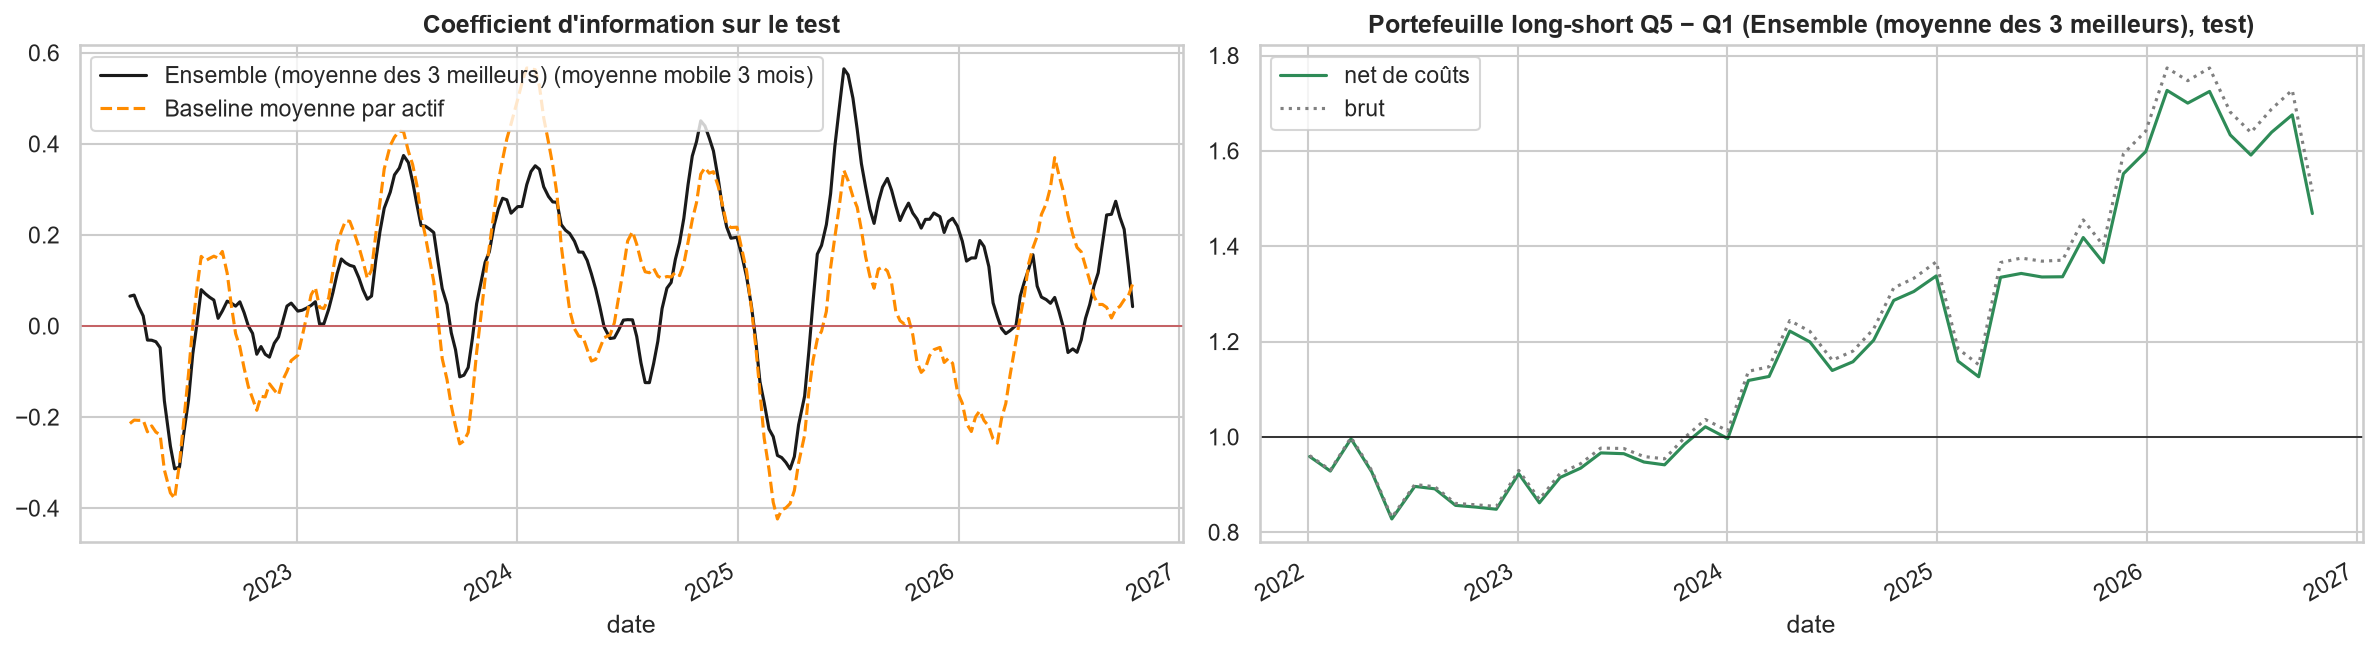
\includegraphics[width=\textwidth]{11_prevision_test.png}
  \caption{Sur le test : coefficient d'information (moyenne mobile sur trois mois) et valeur cumulée du portefeuille long-short Q5-Q1 construit avec l'ensemble.}
  \label{fig:prev_test}
\end{figure}

Ces résultats appellent trois commentaires.

\paragraph{La dérive des données s'est produite.} La référence \og moyenne par actif \fg{}, la meilleure sur 2013-2021, devient nettement moins bonne que la prévision nulle ($R^2 = -9{,}8$ \%). La prime de classe d'actifs s'est retournée en 2022, quand actions et obligations ont baissé ensemble. C'est exactement le risque annoncé par l'analyse exploratoire.

\paragraph{L'ensemble ne prévoit pas mieux les rendements.} Sa MSE est identique à celle de la prévision nulle ($R^2 = 0{,}15$ \%, $p = 0{,}94$). Le garde-fou a eu raison sur le critère qu'il s'était fixé.

\paragraph{Mais il classe un peu les actifs.} Son IC est de 0,10, significatif ($t = 2{,}35$), et le portefeuille long-short qui en découle gagne 9,8 \% par an après coûts. Faut-il en conclure qu'il aurait fallu l'activer ? Nous pensons que non, pour deux raisons. D'abord, l'IC a été très instable (négatif en 2022, autour de 0,17 de 2023 à 2025, proche de zéro en 2026) ; le simple momentum 12-1, sans apprentissage, fait presque aussi bien (9,4 \%). Ensuite, et surtout, changer la règle \emph{après} avoir vu le test reviendrait à utiliser le test pour décider : c'est précisément la fuite que tout notre protocole cherche à éviter. Le résultat est noté comme une piste : un critère fondé sur le classement (l'IC) plutôt que sur l'erreur quadratique pourrait être plus adapté à l'usage qu'on fait des prévisions. Il faudrait le valider sur une nouvelle période.

\subsection{Explicabilité et analyse des erreurs}

Les variables qui comptent le plus dans les prévisions (valeurs SHAP moyennes sur le test) sont les rendements passés à 3, 6 et 12 mois, le momentum 12-1 et les volatilités à 1 et 3 mois : le modèle combine un effet de tendance et un effet de risque. L'analyse par classe d'actifs montre que le modèle prévoit le bon \emph{sens} des écarts (rendement excédentaire prévu négatif pour les obligations et le monétaire, positif pour les actions et le Bitcoin) mais avec une amplitude bien plus faible que la réalité. C'est le comportement attendu d'un modèle fortement régularisé : il ramène ses prévisions vers zéro faute de confiance dans le signal.

En résumé, l'agent Prévision a été construit avec soin, évalué honnêtement et désactivé par une règle décidée à l'avance. Ce résultat négatif est, à nos yeux, l'un des apports du projet : il montre qu'un système d'apprentissage automatique doit savoir \emph{renoncer} à une prévision quand rien ne prouve qu'elle est utile.
